\chapter{Haces Con Momentum Orbital Angular}

\begin{figure}[H]
	\centering
	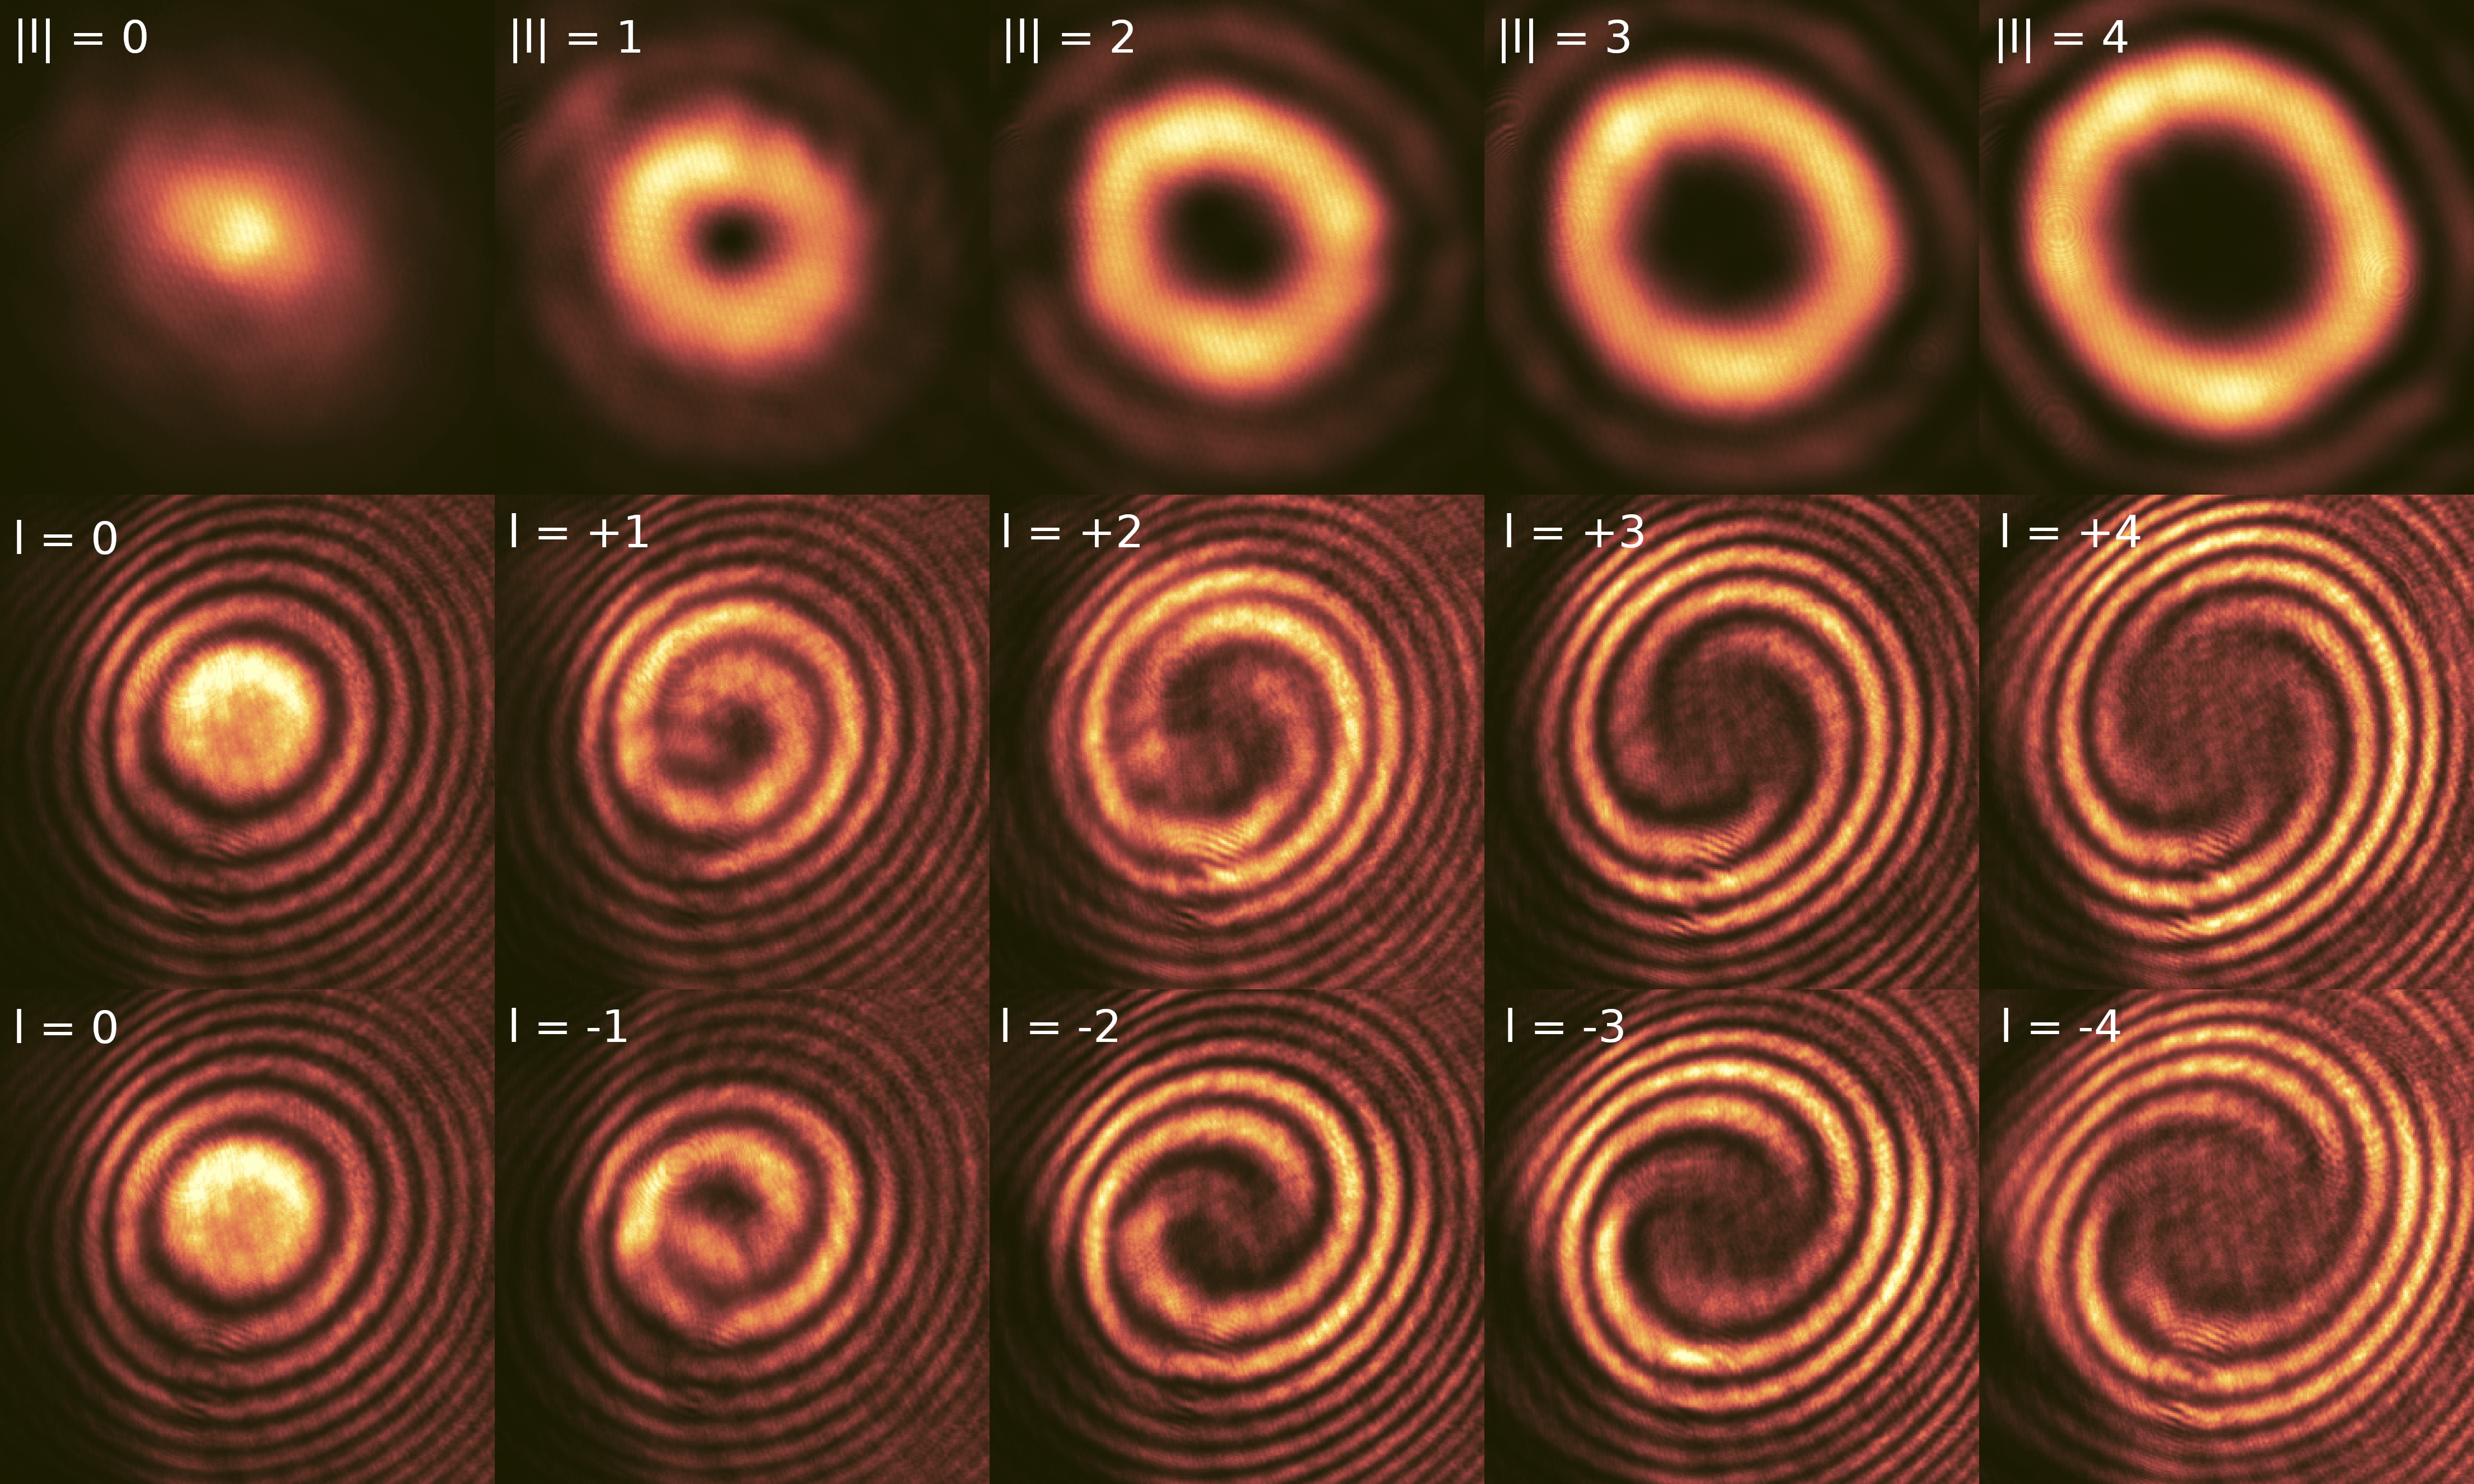
\includegraphics[width=0.8\linewidth]{media/OAM-free.png}
	\caption[Generación de OAMs e interferencia tipo Mach-Zehnder.]{Generación de OAMs e interferencia tipo Mach-Zehnder. Se aprecia la carga de los OAMs contando la cantidad de espirales originados desde el centro.}
\end{figure}

\begin{figure}[H]
	\centering
	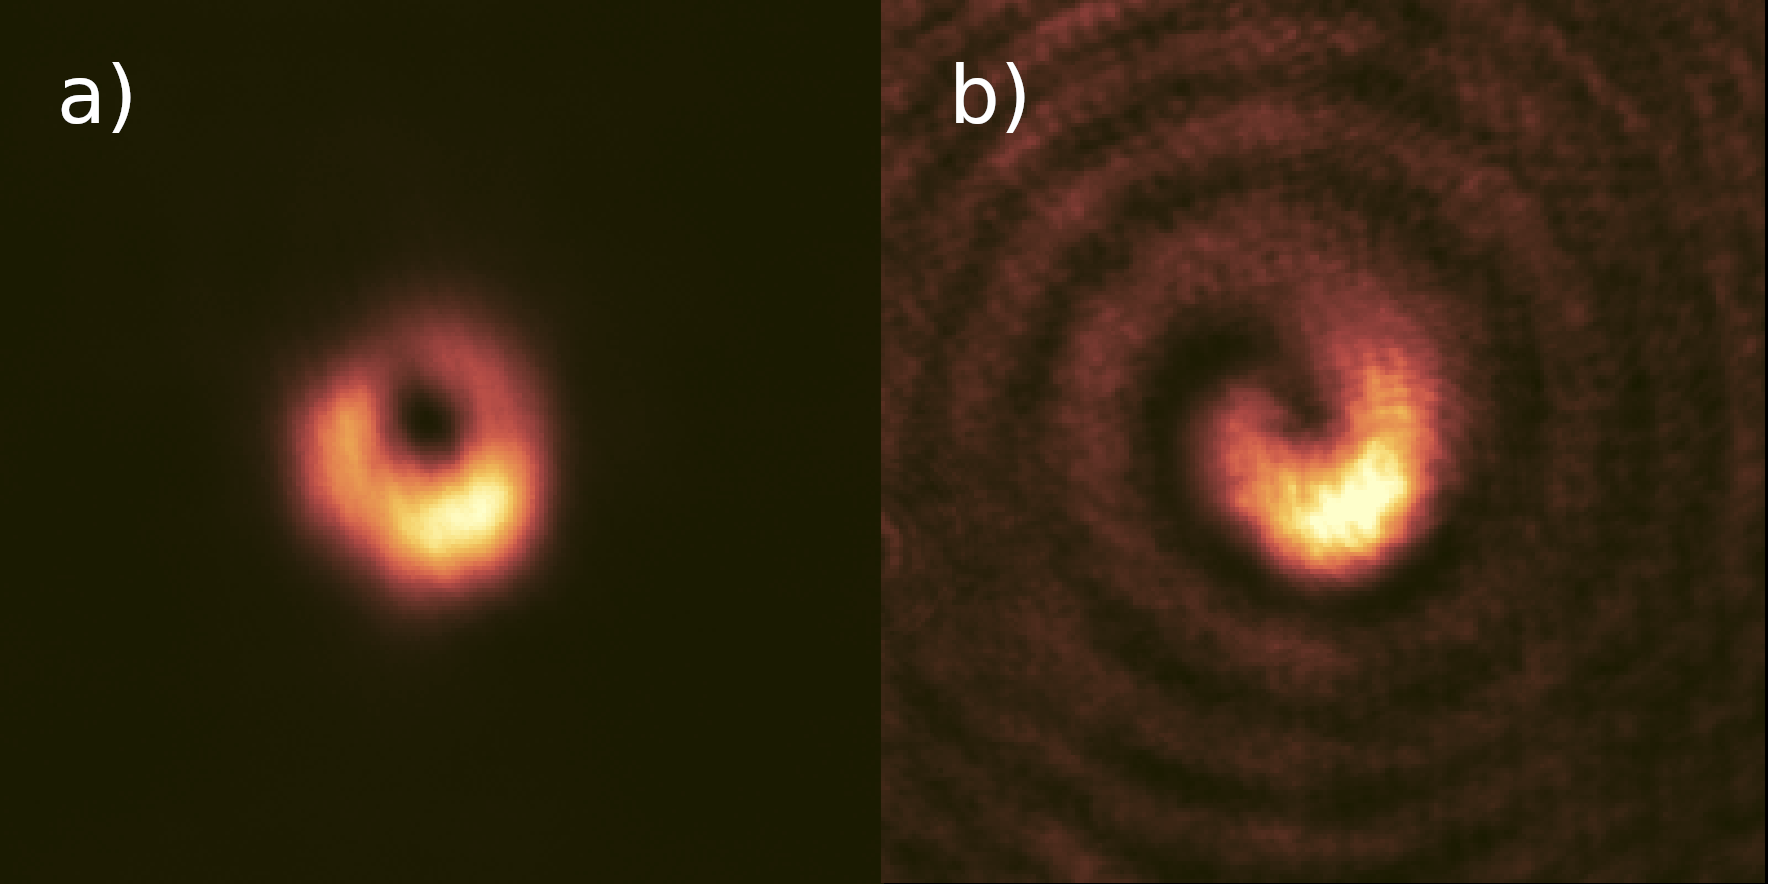
\includegraphics[width=0.8\linewidth]{media/vortex.png}
	\caption[Propagación de vórtices en guías de onda.]{Propagación de vórtices en guías de onda. En a) se tiene la intensidad del perfil de salida luego de excitar un OAM con carga $\ell=1$. En b) se tiene una estructura de fase \textcolor{red}{similar a la esperada pero con falta de definición}.}
\end{figure}